% RustKernels Executive Overview
% Compile with: pdflatex rustkernels-executive-overview.tex (run twice for TOC)
\documentclass[11pt,a4paper]{article}

% ── Packages ──────────────────────────────────────────────────────────────────
\usepackage[utf8]{inputenc}
\usepackage[T1]{fontenc}
\usepackage{lmodern}
\usepackage[margin=2.4cm]{geometry}
\usepackage{graphicx}
\usepackage{xcolor}
\usepackage{titlesec}
\usepackage{enumitem}
\usepackage{booktabs}
\usepackage{tabularx}
\usepackage{colortbl}
\usepackage{multirow}
\usepackage{fancyhdr}
\usepackage{hyperref}
\usepackage{amssymb}
\usepackage{tcolorbox}
\usepackage{tikz}
\usepackage{pgfplots}
\pgfplotsset{compat=1.18}
\usetikzlibrary{arrows.meta, positioning, calc, shapes.geometric, backgrounds, fit}

% ── Colours ───────────────────────────────────────────────────────────────────
\definecolor{brand}{HTML}{1A2744}      % Deep navy
\definecolor{accent}{HTML}{D2691E}     % Burnt orange
\definecolor{highlight}{HTML}{E8850C}  % Warm amber
\definecolor{success}{HTML}{2D936C}    % Green
\definecolor{lightbg}{HTML}{FDF6EE}    % Warm light background
\definecolor{midgray}{HTML}{6C757D}    % Muted text

% ── Heading styles ────────────────────────────────────────────────────────────
\titleformat{\section}
  {\Large\bfseries\color{brand}}
  {\thesection}{1em}{}[\vspace{-0.4em}\textcolor{accent}{\rule{\textwidth}{1.2pt}}]

\titleformat{\subsection}
  {\large\bfseries\color{brand}}
  {\thesubsection}{0.8em}{}

\titleformat{\subsubsection}
  {\normalsize\bfseries\color{accent}}
  {\thesubsubsection}{0.6em}{}

% ── Header / Footer ──────────────────────────────────────────────────────────
\pagestyle{fancy}
\fancyhf{}
\renewcommand{\headrulewidth}{0.4pt}
\fancyhead[L]{\small\textcolor{midgray}{RustKernels --- Executive Overview}}
\fancyhead[R]{\small\textcolor{midgray}{v0.3.1}}
\fancyfoot[C]{\small\textcolor{midgray}{\thepage}}

% ── Custom boxes ──────────────────────────────────────────────────────────────
\tcbset{
  keybox/.style={
    colback=lightbg, colframe=accent, boxrule=0.6pt,
    arc=3pt, left=8pt, right=8pt, top=6pt, bottom=6pt,
    colbacktitle=accent, coltitle=white,
    fonttitle=\bfseries, title=#1
  },
  statbox/.style={
    colback=white, colframe=brand, boxrule=0.8pt,
    arc=4pt, left=6pt, right=6pt, top=4pt, bottom=4pt,
    width=0.30\textwidth
  }
}

% ── Hyperref setup ────────────────────────────────────────────────────────────
\hypersetup{
  colorlinks=true,
  linkcolor=brand,
  urlcolor=accent,
  citecolor=brand,
  pdftitle={RustKernels -- GPU-Accelerated Kernel Library for Financial Services},
  pdfauthor={Michael Ivertowski},
  pdfsubject={Executive Overview},
}

% ══════════════════════════════════════════════════════════════════════════════
\begin{document}

% ── Title page ────────────────────────────────────────────────────────────────
\begin{titlepage}
\begin{tikzpicture}[remember picture, overlay]
  % Background gradient bar
  \fill[brand] (current page.north west) rectangle
    ([yshift=-9cm]current page.north east);
  % Accent stripe
  \fill[accent] ([yshift=-9cm]current page.north west) rectangle
    ([yshift=-9.4cm]current page.north east);
  % Decorative dots
  \foreach \x in {0.5,1.0,...,5.0} {
    \foreach \y in {0.5,1.0,...,3.0} {
      \fill[white, opacity=0.04] ([xshift=\x cm, yshift=-\y cm]current page.north west)
        circle (1.5pt);
    }
  }
\end{tikzpicture}

\vspace*{1.5cm}
\begin{flushleft}
  {\fontsize{36}{42}\selectfont\bfseries\textcolor{white}{RustKernels}}\\[0.5em]
  {\fontsize{16}{20}\selectfont\textcolor{white!85}{GPU-Accelerated Kernel Library}}\\[0.3em]
  {\large\textcolor{white!65}{Financial Services, Analytics \& Compliance Workloads}}\\[0.3em]
  {\normalsize\textcolor{white!50}{Rust \textbullet{} RingKernel Runtime \textbullet{} Batch \& Ring Execution \textbullet{} REST/gRPC API}}
\end{flushleft}

\vspace{5.5cm}

\begin{flushleft}
  \textcolor{midgray}{\large Executive Overview}\\[0.8em]
  {\Large\textcolor{brand}{\textbf{Version 0.3.1}}}\\[1.5em]
  \textcolor{midgray}{%
    106 GPU-accelerated kernels across 14 domains with enterprise\\
    security, observability, resilience, and service APIs ---\\
    built on the RustCompute (RingKernel) framework.%
  }
\end{flushleft}

\vfill
\begin{flushleft}
  \textcolor{midgray}{\small
    Built with Rust \textbullet{} 19 modular crates \textbullet{} Sub-microsecond Ring latency\\[4pt]
    Proprietary (All Rights Reserved) \textbullet{} Enterprise license\\[4pt]
    \textbf{Contact:} \href{mailto:michael.ivertowski@ch.ey.com}{michael.ivertowski@ch.ey.com}
  }
\end{flushleft}
\end{titlepage}

% ── Table of Contents ─────────────────────────────────────────────────────────
\tableofcontents
\newpage

% ══════════════════════════════════════════════════════════════════════════════
\section{Executive Summary}

RustKernels is a GPU-accelerated kernel library purpose-built for financial
services, analytics, and compliance workloads. It is a Rust port of the
DotCompute GPU kernel library, built on the RustCompute (RingKernel) framework,
delivering 106 production-ready kernels across 14 business domains with both
Batch and Ring execution modes.

\begin{tcolorbox}[keybox={Why RustKernels?}]
\begin{itemize}[leftmargin=1.2em, itemsep=3pt]
  \item \textbf{Dual execution modes} --- Batch kernels for heavy periodic
        computation (10--50\,$\mu$s launch) and Ring kernels as GPU-persistent
        actors with 100--500\,ns message latency.
  \item \textbf{14 business domains} --- comprehensive coverage from graph
        analytics and ML to compliance, risk, banking, treasury, and audit.
  \item \textbf{Enterprise-ready} --- built-in security (JWT, RBAC,
        multi-tenancy), observability (Prometheus, OTLP tracing), and
        resilience (circuit breakers, retry, timeouts).
  \item \textbf{Service APIs} --- deploy as a standalone service via Axum
        REST, Tonic gRPC, Tower middleware, or Actix actors.
  \item \textbf{Memory safety} --- Rust's ownership model eliminates data
        races in GPU-host coordination without sacrificing performance.
  \item \textbf{Iterative \& checkpointable} --- multi-pass algorithms
        (PageRank, K-Means) with convergence tracking and graceful
        degradation under load.
\end{itemize}
\end{tcolorbox}

\subsection{At a Glance}

\vspace{0.6em}
\begin{center}
\begin{tabular}{@{}c@{\hspace{1.8em}}c@{\hspace{1.8em}}c@{}}
% Row 1
\begin{tcolorbox}[statbox, width=4.8cm]
  \centering
  {\fontsize{26}{30}\selectfont\bfseries\textcolor{accent}{106}}\\[3pt]
  {\small GPU-accelerated kernels}
\end{tcolorbox} &
\begin{tcolorbox}[statbox, width=4.8cm]
  \centering
  {\fontsize{26}{30}\selectfont\bfseries\textcolor{accent}{14}}\\[3pt]
  {\small business domains}
\end{tcolorbox} &
\begin{tcolorbox}[statbox, width=4.8cm]
  \centering
  {\fontsize{26}{30}\selectfont\bfseries\textcolor{accent}{19}}\\[3pt]
  {\small modular Rust crates}
\end{tcolorbox} \\[0.8em]
% Row 2
\begin{tcolorbox}[statbox, width=4.8cm]
  \centering
  {\fontsize{26}{30}\selectfont\bfseries\textcolor{accent}{$<$500\,ns}}\\[3pt]
  {\small Ring message latency}
\end{tcolorbox} &
\begin{tcolorbox}[statbox, width=4.8cm]
  \centering
  {\fontsize{26}{30}\selectfont\bfseries\textcolor{accent}{2}}\\[3pt]
  {\small execution modes}
\end{tcolorbox} &
\begin{tcolorbox}[statbox, width=4.8cm]
  \centering
  {\fontsize{26}{30}\selectfont\bfseries\textcolor{accent}{4}}\\[3pt]
  {\small service integrations}
\end{tcolorbox}
\end{tabular}
\end{center}

% ══════════════════════════════════════════════════════════════════════════════
\newpage
\section{Execution Modes}

RustKernels provides two complementary execution modes, each optimized for
different latency and throughput requirements.

\subsection{Batch Kernels}

\begin{table}[h!]
\centering
\renewcommand{\arraystretch}{1.25}
\begin{tabularx}{\textwidth}{>{\bfseries\color{brand}}l X}
\toprule
\rowcolor{accent} \textcolor{white}{\textbf{Property}} & \textcolor{white}{\textbf{Details}} \\
\midrule
Launch Overhead & 10--50\,$\mu$s per invocation \\
State Location & CPU memory, launched on-demand \\
Orchestration & CPU-orchestrated dispatch to GPU \\
Best For & Heavy periodic computation, analytics pipelines, report generation \\
Trait & \texttt{BatchKernel<I, O>} with \texttt{execute()} and \texttt{execute\_with\_context()} \\
\bottomrule
\end{tabularx}
\end{table}

\subsection{Ring Kernels}

\begin{table}[h!]
\centering
\renewcommand{\arraystretch}{1.25}
\begin{tabularx}{\textwidth}{>{\bfseries\color{brand}}l X}
\toprule
\rowcolor{accent} \textcolor{white}{\textbf{Property}} & \textcolor{white}{\textbf{Details}} \\
\midrule
Message Latency & 100--500\,ns per message \\
State Location & Permanently in GPU memory \\
Orchestration & GPU-persistent actors, always running \\
Best For & High-frequency operations, real-time streaming, order matching \\
Trait & \texttt{RingKernelHandler<M, R>} with \texttt{handle()} and \texttt{handle\_secure()} \\
\bottomrule
\end{tabularx}
\end{table}

\subsection{Specialized Traits}

Beyond the two primary execution modes, kernels can implement additional
traits for advanced behavior:

\begin{itemize}[leftmargin=1.4em, itemsep=2pt]
  \item \textbf{IterativeKernel} --- multi-pass algorithms (PageRank, K-Means)
        with convergence tracking and configurable thresholds.
  \item \textbf{CheckpointableKernel} --- serialize and restore kernel state
        for recovery after failures or planned restarts.
  \item \textbf{DegradableKernel} --- graceful degradation under load with
        configurable degradation levels.
\end{itemize}

\subsection{K2K Messaging}

Kernel-to-Kernel (K2K) coordination enables complex multi-kernel workflows
via four patterns:
\textbf{IterativeState} (convergence tracking),
\textbf{ScatterGather} (parallel workers),
\textbf{FanOut} (broadcast), and
\textbf{Pipeline} (multi-stage processing).

% ══════════════════════════════════════════════════════════════════════════════
\newpage
\section{Domain Kernels}

RustKernels organizes 106 kernels across 14 business domains, each in its own
crate with dedicated message types, ring messages, and comprehensive tests.

\subsection{Domain Overview}

\begin{table}[h!]
\centering
\renewcommand{\arraystretch}{1.25}
\begin{tabularx}{\textwidth}{>{\bfseries\color{brand}}l c X}
\toprule
\rowcolor{accent} \textcolor{white}{\textbf{Domain}} & \textcolor{white}{\textbf{Kernels}} & \textcolor{white}{\textbf{Key Capabilities}} \\
\midrule
Graph Analytics & 28 &
  PageRank, community detection, GNN inference, graph attention,
  centrality, pathfinding, connected components. \\
Statistical ML & 17 &
  Embedding generation, semantic similarity, SHAP values,
  feature importance, isolation forest, adaptive thresholds. \\
Compliance & 11 &
  Regulatory scanning, sanctions screening, transaction monitoring,
  audit trail validation. \\
Temporal Analysis & 7 &
  Time-series decomposition, trend detection, seasonality analysis,
  change-point detection. \\
Process Intelligence & 7 &
  Digital twin simulation, next-activity prediction, event log
  imputation, process conformance. \\
Behavioral Analytics & 6 &
  User behavior profiling, session analysis, anomaly detection,
  interaction patterns. \\
Risk Analytics & 5 &
  VaR calculation, stress testing, risk aggregation, exposure
  analysis. \\
Clearing & 5 &
  Netting, settlement, margin calculation, position reconciliation. \\
Treasury & 5 &
  Cash flow forecasting, liquidity management, FX exposure,
  investment analytics. \\
Accounting & 9 &
  Journal entry validation, trial balance, reconciliation,
  period close, consolidation. \\
Payments & 2 &
  Payment processing, fraud scoring. \\
Audit & 2 &
  Audit sampling, evidence evaluation. \\
Banking & 1 &
  Core banking transaction processing. \\
Order Matching & 1 &
  High-frequency order book matching engine. \\
\bottomrule
\end{tabularx}
\end{table}

\subsection{Domain Crate Structure}

Each domain crate follows a consistent, self-contained structure:

\begin{tcolorbox}[colback=brand!3, colframe=brand!40, boxrule=0.5pt, arc=3pt,
                   left=8pt, right=8pt, top=6pt, bottom=6pt]
\ttfamily\small
rustkernel-\{domain\}/\\
\quad src/\\
\quad\quad lib.rs \hfill \textrm{\textcolor{midgray}{\small Module exports, register\_all()}}\\
\quad\quad messages.rs \hfill \textrm{\textcolor{midgray}{\small Batch kernel input/output types}}\\
\quad\quad ring\_messages.rs \hfill \textrm{\textcolor{midgray}{\small Ring message types with \#[derive(RingMessage)]}}\\
\quad\quad types.rs \hfill \textrm{\textcolor{midgray}{\small Common domain types}}\\
\quad\quad \{feature\}.rs \hfill \textrm{\textcolor{midgray}{\small Kernel implementations}}
\end{tcolorbox}

\noindent
\textbf{Ring Message Type ID Ranges:}
Each domain has a reserved range to prevent collisions ---
\textbf{Graph}\,200--299,
\textbf{Compliance}\,300--399,
\textbf{Temporal}\,400--499,
\textbf{Risk}\,600--699,
\textbf{ML}\,700--799.

% ══════════════════════════════════════════════════════════════════════════════
\newpage
\section{Featured Kernels}

\subsection{Graph Analytics}

\begin{table}[h!]
\centering
\renewcommand{\arraystretch}{1.2}
\begin{tabularx}{\textwidth}{>{\bfseries\color{brand}}l X}
\toprule
\rowcolor{accent} \textcolor{white}{\textbf{Kernel}} & \textcolor{white}{\textbf{Description}} \\
\midrule
PageRank &
  Iterative link analysis with configurable damping factor and
  convergence threshold. Implements \texttt{IterativeKernel}. \\
GNN Inference &
  Message-passing neural network inference for node classification
  and link prediction on transaction graphs. \\
Graph Attention &
  Graph Attention Network with multi-head attention for learning
  node representations with weighted neighbor aggregation. \\
Community Detection &
  Louvain and label propagation algorithms for discovering
  clusters in entity relationship graphs. \\
\bottomrule
\end{tabularx}
\end{table}

\subsection{Machine Learning}

\begin{table}[h!]
\centering
\renewcommand{\arraystretch}{1.2}
\begin{tabularx}{\textwidth}{>{\bfseries\color{brand}}l X}
\toprule
\rowcolor{accent} \textcolor{white}{\textbf{Kernel}} & \textcolor{white}{\textbf{Description}} \\
\midrule
SHAP Values &
  Kernel SHAP implementation for model-agnostic feature attribution
  and explainability on GPU. \\
Secure Aggregation &
  Federated learning aggregation with differential privacy for
  privacy-preserving model training. \\
Streaming Isolation Forest &
  Online anomaly detection with adaptive tree updates for
  real-time transaction monitoring. \\
Adaptive Threshold &
  Self-adjusting thresholds with concept drift detection for
  evolving data distributions. \\
Drug Interaction &
  Multi-drug interaction prediction using molecular fingerprints
  and interaction scoring. \\
\bottomrule
\end{tabularx}
\end{table}

\subsection{Process Intelligence}

\begin{table}[h!]
\centering
\renewcommand{\arraystretch}{1.2}
\begin{tabularx}{\textwidth}{>{\bfseries\color{brand}}l X}
\toprule
\rowcolor{accent} \textcolor{white}{\textbf{Kernel}} & \textcolor{white}{\textbf{Description}} \\
\midrule
Digital Twin &
  Monte Carlo process simulation for capacity planning, bottleneck
  identification, and what-if analysis. \\
Next Activity Prediction &
  Markov chain and N-gram models for predicting the next activity
  in a business process execution. \\
Event Log Imputation &
  Automated detection and repair of missing, out-of-order, and
  duplicate events in process logs. \\
\bottomrule
\end{tabularx}
\end{table}

% ══════════════════════════════════════════════════════════════════════════════
\newpage
\section{Enterprise Modules}

RustKernels v0.3.1 includes five enterprise modules providing production-grade
infrastructure for deployment at scale.

\subsection{Security}

\begin{table}[h!]
\centering
\renewcommand{\arraystretch}{1.2}
\begin{tabularx}{\textwidth}{>{\bfseries\color{brand}}l X}
\toprule
\rowcolor{accent} \textcolor{white}{\textbf{Feature}} & \textcolor{white}{\textbf{Details}} \\
\midrule
Authentication &
  JWT and API key validation via \texttt{AuthConfig} with pluggable
  providers. \\
RBAC &
  Role-based access control with four permission levels: Execute,
  Configure, Monitor, Admin. \\
Multi-Tenancy &
  Tenant isolation with \texttt{TenantId}, resource quotas, and
  per-tenant kernel registries. \\
Secrets &
  \texttt{SecretStore} abstraction for credential management with
  environment and vault backends. \\
\bottomrule
\end{tabularx}
\end{table}

\subsection{Observability}

\begin{table}[h!]
\centering
\renewcommand{\arraystretch}{1.2}
\begin{tabularx}{\textwidth}{>{\bfseries\color{brand}}l X}
\toprule
\rowcolor{accent} \textcolor{white}{\textbf{Feature}} & \textcolor{white}{\textbf{Details}} \\
\midrule
Metrics &
  Prometheus-compatible metrics via \texttt{KernelMetrics} with
  histograms, counters, and gauges per kernel. \\
Tracing &
  Distributed tracing with OTLP export via \texttt{KernelTracing},
  span propagation across K2K calls. \\
Logging &
  Structured logging with kernel context, tenant ID, and
  correlation IDs. \\
Alerting &
  SLO-based alerts with configurable \texttt{AlertRule} definitions
  and notification channels. \\
\bottomrule
\end{tabularx}
\end{table}

\subsection{Resilience}

\begin{table}[h!]
\centering
\renewcommand{\arraystretch}{1.2}
\begin{tabularx}{\textwidth}{>{\bfseries\color{brand}}l X}
\toprule
\rowcolor{accent} \textcolor{white}{\textbf{Feature}} & \textcolor{white}{\textbf{Details}} \\
\midrule
Circuit Breaker &
  Failure isolation with configurable thresholds, half-open probing,
  and automatic recovery. \\
Retry &
  Exponential backoff with jitter, configurable max attempts, and
  per-kernel retry policies. \\
Timeouts &
  Deadline propagation with \texttt{DeadlineContext} ensuring
  cascading timeout enforcement. \\
Health Checks &
  Liveness and readiness probes via \texttt{HealthProbe} with
  per-kernel health status reporting. \\
\bottomrule
\end{tabularx}
\end{table}

% ══════════════════════════════════════════════════════════════════════════════
\newpage
\subsection{Runtime \& Memory}

\begin{table}[h!]
\centering
\renewcommand{\arraystretch}{1.2}
\begin{tabularx}{\textwidth}{>{\bfseries\color{brand}}l X}
\toprule
\rowcolor{accent} \textcolor{white}{\textbf{Feature}} & \textcolor{white}{\textbf{Details}} \\
\midrule
Lifecycle &
  State machine with Starting $\to$ Running $\to$ Draining $\to$
  Stopped transitions and graceful shutdown. \\
Configuration &
  \texttt{RuntimeConfig} with presets: development, production,
  high-performance; file and environment sources. \\
Memory Pooling &
  Size-stratified memory pools via \texttt{KernelMemoryManager}
  with configurable pressure thresholds. \\
GPU Reductions &
  Multi-phase GPU reductions via \texttt{InterPhaseReduction} for
  efficient large-scale aggregation. \\
Analytics Contexts &
  Workload-specific buffer management with
  \texttt{AnalyticsContextManager}. \\
\bottomrule
\end{tabularx}
\end{table}

\subsection{Licensing}

Enterprise licensing with domain-based validation:

\begin{itemize}[leftmargin=1.4em, itemsep=2pt]
  \item \textbf{DevelopmentLicense} --- all features enabled for local
        development and testing.
  \item \textbf{Domain-based gating} --- feature validation at kernel
        registration and activation time via \texttt{LicenseValidator}.
  \item \textbf{Per-kernel control} --- individual kernel enablement with
        license tier awareness.
\end{itemize}

% ══════════════════════════════════════════════════════════════════════════════
\section{Service Integrations}

The \texttt{rustkernel-ecosystem} crate provides four service integration
paths for deploying RustKernels as a standalone service.

\begin{center}
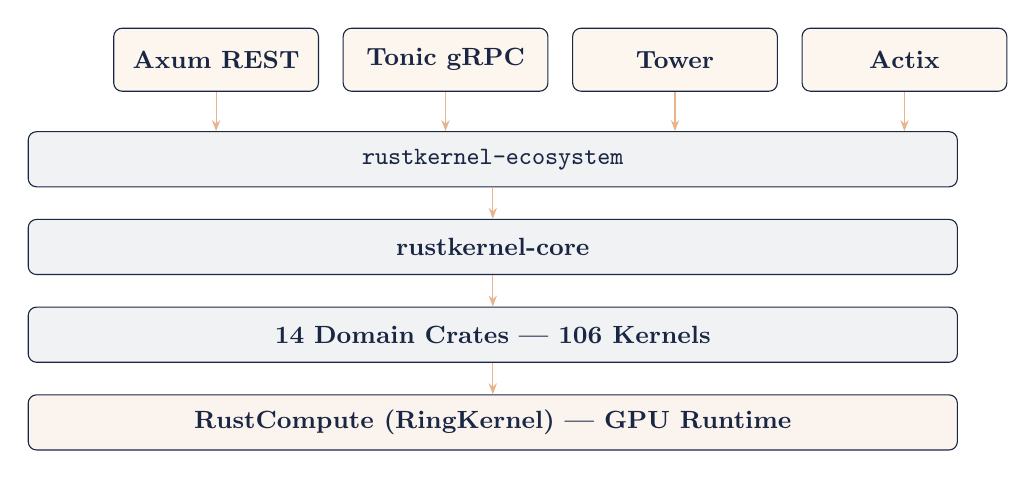
\begin{tikzpicture}[
  node distance=0.5cm,
  box/.style={draw=brand, fill=lightbg, rounded corners=3pt,
              minimum width=2.6cm, minimum height=0.8cm,
              font=\small\bfseries, text=brand, align=center},
  wide/.style={draw=brand, fill=brand!6, rounded corners=3pt,
               minimum width=11.8cm, minimum height=0.7cm,
               font=\small\bfseries, text=brand, align=center},
  arr/.style={-{Stealth[length=4pt]}, color=accent!50}
]
  % Service layer
  \node[box] (axum) {Axum REST};
  \node[box, right=0.3cm of axum] (tonic) {Tonic gRPC};
  \node[box, right=0.3cm of tonic] (tower) {Tower};
  \node[box, right=0.3cm of tower] (actix) {Actix};

  \node[wide, below=0.5cm of tonic, xshift=0.6cm]
    (eco) {\texttt{rustkernel-ecosystem}};
  \node[wide, below=0.4cm of eco]
    (core) {\textbf{rustkernel-core}};
  \node[wide, below=0.4cm of core]
    (domains) {14 Domain Crates --- 106 Kernels};
  \node[wide, below=0.4cm of domains, fill=accent!8]
    (ring) {\textbf{RustCompute (RingKernel)} --- GPU Runtime};

  \draw[arr] (axum.south) -- (axum.south |- eco.north);
  \draw[arr] (tonic.south) -- (tonic.south |- eco.north);
  \draw[arr] (tower.south) -- (tower.south |- eco.north);
  \draw[arr] (actix.south) -- (actix.south |- eco.north);
  \draw[arr] (eco.south) -- (core.north);
  \draw[arr] (core.south) -- (domains.north);
  \draw[arr] (domains.south) -- (ring.north);
\end{tikzpicture}
\end{center}

\begin{table}[h!]
\centering
\renewcommand{\arraystretch}{1.2}
\begin{tabularx}{\textwidth}{>{\bfseries\color{brand}}l X}
\toprule
\rowcolor{accent} \textcolor{white}{\textbf{Integration}} & \textcolor{white}{\textbf{Details}} \\
\midrule
Axum REST &
  \texttt{KernelRouter} with endpoints: \texttt{/kernels},
  \texttt{/execute}, \texttt{/health}, \texttt{/metrics}. \\
Tonic gRPC &
  \texttt{KernelGrpcServer} for high-performance RPC with
  protobuf serialization. \\
Tower Middleware &
  \texttt{TimeoutLayer}, \texttt{RateLimiterLayer}, and
  \texttt{KernelService} for composable request pipelines. \\
Actix Actors &
  \texttt{KernelActor} for actor-based concurrency and message-driven
  kernel execution. \\
\bottomrule
\end{tabularx}
\end{table}

% ══════════════════════════════════════════════════════════════════════════════
\newpage
\section{Architecture}

\subsection{Workspace Structure}

\begin{center}
\resizebox{\textwidth}{!}{%
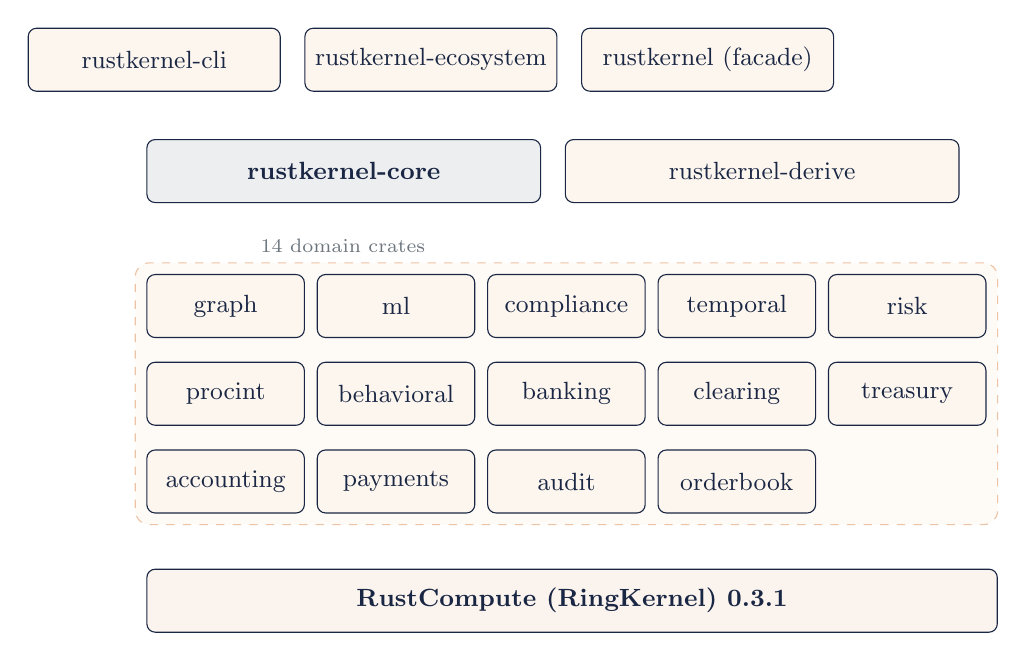
\begin{tikzpicture}[
  node distance=0.4cm,
  layer/.style={draw=brand, fill=lightbg, rounded corners=3pt,
                minimum height=0.8cm, font=\small, text=brand, align=center},
  wide/.style={draw=brand, rounded corners=3pt,
               minimum height=0.8cm, font=\small, text=brand, align=center},
]
  % Top layer --- interfaces
  \node[layer, minimum width=3.2cm] (cli) {rustkernel-cli};
  \node[layer, minimum width=3.2cm, right=0.3cm of cli] (eco) {rustkernel-ecosystem};
  \node[layer, minimum width=3.2cm, right=0.3cm of eco] (facade) {rustkernel (facade)};

  % Core + Derive
  \node[layer, minimum width=5.0cm, below=0.6cm of cli, anchor=north west,
        xshift=-0.1cm, fill=brand!8]
    (core) {\textbf{rustkernel-core}};
  \node[layer, minimum width=5.0cm, right=0.3cm of core]
    (derive) {rustkernel-derive};

  % Domain crates --- grouped in a fitted box
  \node[layer, minimum width=2.0cm, below=0.9cm of core.south west,
        anchor=north west] (graph) {graph};
  \node[layer, minimum width=2.0cm, right=0.15cm of graph] (ml) {ml};
  \node[layer, minimum width=2.0cm, right=0.15cm of ml] (compliance) {compliance};
  \node[layer, minimum width=2.0cm, right=0.15cm of compliance] (temporal) {temporal};
  \node[layer, minimum width=2.0cm, right=0.15cm of temporal] (risk) {risk};

  \node[layer, minimum width=2.0cm, below=0.3cm of graph] (procint) {procint};
  \node[layer, minimum width=2.0cm, right=0.15cm of procint] (behavioral) {behavioral};
  \node[layer, minimum width=2.0cm, right=0.15cm of behavioral] (banking) {banking};
  \node[layer, minimum width=2.0cm, right=0.15cm of banking] (clearing) {clearing};
  \node[layer, minimum width=2.0cm, right=0.15cm of clearing] (treasury) {treasury};

  \node[layer, minimum width=2.0cm, below=0.3cm of procint] (accounting) {accounting};
  \node[layer, minimum width=2.0cm, right=0.15cm of accounting] (payments) {payments};
  \node[layer, minimum width=2.0cm, right=0.15cm of payments] (audit) {audit};
  \node[layer, minimum width=2.0cm, right=0.15cm of audit] (orderbook) {orderbook};

  % Fit box around domain crates
  \begin{scope}[on background layer]
    \node[draw=accent!40, dashed, rounded corners=5pt, fill=lightbg!50,
          fit=(graph)(risk)(accounting)(orderbook),
          inner sep=4pt, label={[font=\scriptsize\color{midgray}]above left:14 domain crates}] {};
  \end{scope}

  % RingKernel foundation
  \node[wide, minimum width=10.8cm, below=0.7cm of accounting.south west,
        anchor=north west, fill=accent!8]
    (ringkernel) {\textbf{RustCompute (RingKernel) 0.3.1}};
\end{tikzpicture}%
}% end resizebox
\end{center}

\subsection{Core Trait Hierarchy}

All kernels implement \texttt{GpuKernel} (metadata, validation, health).
Execution traits branch into two paths:

\begin{center}
\small
\begin{tabular}{@{}l@{\quad$\longrightarrow$\quad}l@{\quad$\longrightarrow$\quad}l@{}}
\textbf{\textcolor{brand}{BatchKernel<I,\,O>}} &
\textcolor{accent}{IterativeKernel<S,\,I,\,O>} &
\textcolor{midgray}{DegradableKernel} \\[4pt]
\textbf{\textcolor{brand}{RingKernelHandler<M,\,R>}} &
\textcolor{accent}{CheckpointableKernel} &
\textcolor{midgray}{DegradableKernel} \\
\end{tabular}
\end{center}

% ══════════════════════════════════════════════════════════════════════════════
\newpage
\section{Use Cases}

\begin{tcolorbox}[keybox={Primary Use Cases}]
\begin{description}[leftmargin=1em, labelwidth=1em, font=\color{brand}\bfseries]
  \item[$\blacktriangleright$] \textbf{Transaction Graph Analytics} ---
    GPU-accelerated PageRank, community detection, and GNN inference
    on large-scale financial transaction networks.

  \item[$\blacktriangleright$] \textbf{Real-Time Compliance Screening} ---
    Sub-microsecond sanctions screening and transaction monitoring
    via Ring kernels for continuous compliance.

  \item[$\blacktriangleright$] \textbf{Risk Analytics} ---
    VaR calculation, stress testing, and exposure analysis with
    GPU-parallel Monte Carlo simulation.

  \item[$\blacktriangleright$] \textbf{ML Model Serving} ---
    GPU-accelerated inference for fraud detection, anomaly scoring,
    and feature importance with SHAP explanations.

  \item[$\blacktriangleright$] \textbf{High-Frequency Order Matching} ---
    Ring kernel-based order book with persistent GPU state for
    ultra-low-latency matching.

  \item[$\blacktriangleright$] \textbf{Process Intelligence} ---
    Digital twin simulation, next-activity prediction, and event log
    quality analysis for operational optimization.

  \item[$\blacktriangleright$] \textbf{Treasury \& Cash Management} ---
    Cash flow forecasting, liquidity optimization, and FX exposure
    management with temporal analytics.

  \item[$\blacktriangleright$] \textbf{Federated Learning} ---
    Privacy-preserving model training with secure aggregation and
    differential privacy across organizational boundaries.
\end{description}
\end{tcolorbox}

% ══════════════════════════════════════════════════════════════════════════════
\section{Getting Started}

\subsection{Build \& Test}

\begin{tcolorbox}[colback=brand!3, colframe=brand!40, boxrule=0.5pt, arc=3pt,
                   left=8pt, right=8pt, top=6pt, bottom=6pt]
\ttfamily\small
\# Build entire workspace\\
cargo build --workspace\\[6pt]
\# Run all tests\\
cargo test --workspace\\[6pt]
\# Build specific domain crate\\
cargo build --package rustkernel-graph\\[6pt]
\# Lint with all features\\
cargo clippy --all-targets --all-features -- -D warnings
\end{tcolorbox}

\subsection{Deploy as REST Service}

\begin{tcolorbox}[colback=brand!3, colframe=brand!40, boxrule=0.5pt, arc=3pt,
                   left=8pt, right=8pt, top=6pt, bottom=6pt]
\ttfamily\small
use rustkernel\_ecosystem::axum::\{KernelRouter, RouterConfig\};\\[6pt]
let router = KernelRouter::new(registry, RouterConfig::default());\\
let app = router.into\_router();\\
// Serve with axum::Server on port 3000
\end{tcolorbox}

\subsection{Production Configuration}

\begin{tcolorbox}[colback=brand!3, colframe=brand!40, boxrule=0.5pt, arc=3pt,
                   left=8pt, right=8pt, top=6pt, bottom=6pt]
\ttfamily\small
use rustkernel\_core::config::\{ProductionConfigBuilder\};\\[6pt]
let config = ProductionConfigBuilder::production()\\
\quad .service\_name("my-service")\\
\quad .environment("staging")\\
\quad .build()?;
\end{tcolorbox}

% ══════════════════════════════════════════════════════════════════════════════
\vspace{1.5em}
\begin{tcolorbox}[keybox={Ecosystem Integration}]
\renewcommand{\arraystretch}{1.4}
\begin{tabularx}{\textwidth}{>{\bfseries\color{brand}}l X}
  RustCompute &
    GPU-native persistent actor model (RingKernel) providing the
    runtime foundation for all kernel execution. \\
  RustGraph &
    GPU-native living graph database leveraging RustKernels for
    graph analytics and ML algorithms. \\
  DataSynth &
    Enterprise synthetic data platform generating test data for
    kernel development and validation. \\
  AssureTwin &
    Native audit intelligence platform consuming RustKernels for
    GPU-accelerated audit analytics. \\
\end{tabularx}
\end{tcolorbox}

\vfill
\begin{center}
\textcolor{midgray}{\rule{0.5\textwidth}{0.4pt}}\\[0.8em]
{\small\textcolor{midgray}{%
  RustKernels v0.3.1 \textbullet{}
  Proprietary (All Rights Reserved) \textbullet{}
  Enterprise license%
}}\\[4pt]
{\small\textcolor{midgray}{%
  \textbf{Contact:} \href{mailto:michael.ivertowski@ch.ey.com}{michael.ivertowski@ch.ey.com}%
}}
\end{center}

\end{document}
